\documentclass[autodetect-engine,dvipdfmx-if-dvi,ja=standard,a4j,jbase=11pt,magstyle=nomag*]{bxjsreport}
% \documentclass[uplatex, dvipdfmx, a4paper, 11ptj, report]{jsbook}
% small japanese font size:     9pt, 10pt, 11pt, 12pt, 14pt, ... (please refer the document of jsclasses)
% word-like japanese font size: 10ptj 10.5ptj, 11ptj, 12ptj (or jbase=xxpt (without 'j') if error is occured)

\usepackage{ifptex,ifxetex,ifluatex}
\ifluatex
    \usepackage{bxcalcux}
    \ltjsetparameter{jacharrange={-2,-3}}
    \usepackage{luatexja-otf}
    \usepackage{bxbase}
\else\ifxetex
    % \usepackage{zxjatype}
    % \usepackage[macros]{zxotf}
    \XeTeXgenerateactualtext=1
    \usepackage{xltxtra}
    \usepackage{bxbase}
\else\ifuptex
    \usepackage{otf}
    \usepackage[prefernoncjk]{pxcjkcat}
    \cjkcategory{sym11,sym18,sym19}{cjk}
    \usepackage[utf8]{inputenc}
    \usepackage{pxbase}
\else\ifstrictptex
    \usepackage{otf}
    \usepackage[utf8]{inputenc}
    \usepackage{pxbase}
\fi\fi\fi\fi

\usepackage[LGR,T2A,T1]{fontenc}

\usepackage{graphicx}
% \usepackage[dvipdfmx]{graphicx}
\usepackage{grffile}

% paper layout setting
\setpagelayout{noheadfoot, left=18.0truemm, right=18.0truemm, top=29.0truemm, bottom=26.0truemm, columnsep=6.5truemm}
% \setpagelayout{noheadfoot, left=15.0truemm, right=5.0truemm, top=12.5truemm, bottom=12.5truemm, columnsep=5.0truemm}

% font setting
\usepackage{amsmath}
\usepackage{amssymb}
\usepackage{mathtools}
\usepackage{bm}
\usepackage{fix-cm}
\usepackage{newtxtext}
\usepackage[slantedGreek]{newtxmath}

% caption setting
\usepackage[font=bf,labelfont=bf,labelsep=quad]{caption}

% to balance the last page of the two-column article
% \usepackage[nospread, keeplastbox, nodebug]{flushend}

% title font style
\renewcommand{\headfont}{\bfseries}

% section setting (using titlesec, uelm package)
\renewcommand{\thesection}{\arabic{section}}
\renewcommand{\thesubsection}{\arabic{section}.\arabic{subsection}}

\usepackage[explicit]{titlesec}
\usepackage[normalem]{ulem}
\titleformat{name=\section}{\normalfont\headfont\normalsize\raggedright}{}{0pt}{\uline{\thesection.\quad#1}}
\titleformat{name=\section,numberless}{\normalfont\headfont\normalsize\raggedright}{}{0pt}{\uline{#1}}
% \titleformat{name=\section}{\normalfont\headfont\normalsize\raggedright}{}{0pt}{\thesection.\quad#1}
\titlespacing{name=\section}{0pt}{.5\Cvs plus .0\Cvs minus .3\Cvs}{.1\Cvs plus .0\Cvs minus .1\Cvs}
\titleformat{name=\subsection}{\normalfont\headfont\normalsize\raggedright}{}{0pt}{\thesubsection.\quad#1}
\titleformat{name=\subsection,numberless}{\normalfont\headfont\normalsize\raggedright}{}{0pt}{#1}
\titlespacing{name=\subsection}{0pt}{.3\Cvs plus .0\Cvs minus .2\Cvs}{.0\Cvs plus .0\Cvs minus .0\Cvs}

% \makeatletter
% \renewcommand{\section}{\@startsection{section}{1}{\z@}{.5\baselineskip}{.1\baselineskip}{\normalfont\normalsize\headfont\raggedright}}
% \renewcommand{\subsection}{\@startsection{subsection}{2}{\z@}{.3\baselineskip}{\z@}{\normalfont\normalsize\headfont\raggedright}}
% \makeatother

\usepackage{secdot}
\sectiondot{section}
\sectiondot{subsection}

% list (itemize, enumerate, description, ...)
\usepackage{enumitem}
\setlist[1]{parsep=.0\baselineskip,topsep=.2\baselineskip,itemsep=.1\baselineskip}
% \makeatletter
% \def\@listi{\leftmargin\leftmargini
%     \parsep \z@
%     \topsep .2\baselineskip
%     \itemsep .1\baselineskip \relax}
% \let\@listI\@listi
% \makeatother

% no page number
\pagestyle{empty}

% footnote
\usepackage[bottom,hang,stable]{footmisc}
\setlength{\footnotemargin}{0pt}

% float setting (figure, table)
\setlength\floatsep{2.0truemm}
\setlength\textfloatsep{2.0truemm}
\setlength\intextsep{1.0truemm}
\setlength\dblfloatsep{2.0truemm}
\setlength\dbltextfloatsep{2.0truemm}
\setlength\abovecaptionskip{0.5truemm}
\setlength\belowcaptionskip{0.5truemm}

% lineskip setting (body text, display-style equation)
\AtBeginDocument{%
    \narrowbaselines    % basic english lineskip (for article)
    % \widebaselines      % basic japanese lineskip
    %
    \setlength\abovedisplayskip{1.5truemm}    % equation setting
    \setlength\belowdisplayskip{1.5truemm}    % equation setting
}

% to suit ms-word template
\renewcommand{\baselinestretch}{0.9}


\makeatletter
%
% maketitle
% additional elements
\newcommand*{\etitle}[1]{\gdef\@etitle{#1}}
\newcommand*{\studentid}[1]{\gdef\@studentid{#1}}
\newcommand*{\laboarea}[1]{\gdef\@laboarea{#1}}
\newcommand*{\laboname}[1]{\gdef\@laboname{#1}}
%
% style definition
\def\@maketitle{%
\newpage%
\centering%
\let\footnote\thanks%
%
% title
{\fontsize{16.00truept}{16.00truept}\selectfont\headfont\@title\par}%
%
% english title
\ifx\@etitle\@undefined\else{\vspace{1truemm}{\fontsize{12truept}{12truept}\selectfont\headfont\@etitle\par}}\fi%
%
% name (option: student id)
\vspace{1truemm}%
\ifx\@studentid\@undefined\else{\fontsize{12truept}{12truept}\selectfont\headfont\@studentid\hspace{\Cwd}}\fi%
{\fontsize{12truept}{12truept}\selectfont\headfont\@author\par}%
%
% research area (\laboarea) and laboratory name (\laboname)
\ifx\@laboarea\@undefined%
    \ifx\@laboname\@undefined%
    \else\vspace{1truemm}{\fontsize{12truept}{12truept}\selectfont\headfont\@laboname\par}%
    \fi%
\else%
    \ifx\@laboname\@undefined\vspace{1truemm}{\fontsize{12truept}{12truept}\selectfont\headfont\@laboarea\par}%
    \else\vspace{1truemm}{\fontsize{12truept}{12truept}\selectfont\headfont\@laboarea\hspace{\Cwd}\@laboname\par}%
    \fi%
\fi%
%
%% old version (2 line) of research area (\laboarea) and laboratory name (\laboname)
%\ifx\@laboarea\@undefined\else{\vspace{1truemm}{\fontsize{10truept}{10truept}\selectfont\@laboarea\par}}\fi%
%\ifx\@laboname\@undefined\else{\vspace{1truemm}{\fontsize{10truept}{10truept}\selectfont\@laboname\par}}\fi%
%
%% date (error)
% \ifvoid\@date\else{\vspace{2truemm}{\fontsize{12truept}{12truept}\selectfont\@date\par}}\fi%
%
% abstract (no check)
\ifvoid\@abstractbox\else{\vspace{2truemm}{\centering{\fontsize{10truept}{10truept}\selectfont\box\@abstractbox\par}}}\fi%
\vspace{2truemm}%
}
%
%
% bibliography
\newcommand{\@bibsection}{\@startsection{section}{1}{\z@}{.5\baselineskip}{0.2\baselineskip}{\normalfont\fontsize{9truept}{11truept}\selectfont\headfont\raggedright}}
\setlength\bibindent{\Cwd}
\renewenvironment{thebibliography}[1]{%
    \global\let\presectionname\relax
    \global\let\postsectionname\relax
    \@bibsection*{\refname}\@mkboth{\refname}{\refname}%
    \list{\@biblabel{\@arabic\c@enumiv}}{%
        \settowidth\labelwidth{\@biblabel{#1}}%
        \leftmargin\labelwidth
        \advance\leftmargin\labelsep
        \setlength\itemsep{0.5truept plus 1.0truept minus 0.5truept}
        \@openbib@code
        \usecounter{enumiv}%
        \let\p@enumiv\@empty
        \renewcommand\theenumiv{\@arabic\c@enumiv}}%
    \fontsize{8truept}{9.5truept}\selectfont
    \sloppy
    \clubpenalty4000
    \@clubpenalty\clubpenalty
    \widowpenalty4000%
    \sfcode`\.\@m}
{\def\@noitemerr{\@latex@warning{Empty `thebibliography' environment}}\endlist}
%
\makeatother


\mainmatter
\setchapterxr[thesis][bibliography]{4}


\begin{document}


\chapter[HRP-2における脚配置計画シミュレーション]{HRP-2における\\脚配置計画シミュレーション}
\label{chap:sim_hrp2}

本章および次章では,提案手法による脚配置計画によって,三次元地形上でどのような計画が得られるのか,
また実時間で計画が行えるかどうかを検証する.
本章および次章で示す結果は,CPU: Intel\textregistered\ Core\texttrademark\ i7-2640M$2.8\,\mathrm{GHz} \times 2$,
RAM:$8\,\mathrm{GB}$のPCを用い,Visual Studio 2013上でVisual C++で作成したプログラムを実行して得られたものである.
計算時間は$100$回計画を行ったときの平均値を示している.

\begin{table}[pt]
    \renewcommand{\arraystretch}{0.9}
    \centering
    % \small
    \caption{Model parameters for HRP-2}
    \label{tab:sim_hrp2_param_model}
    \begin{tabular}{cc}
        \toprule%
        parameters                      &   value \\
        \midrule%
        $z_{\mathrm{max}}$              &   $10.0\,\cm$ \\
        $d_{xy\,\mathrm{max}}$          &   $50.0\,\cm$ \\
        $d_{z\,\mathrm{max}}$           &   $20.0\,\cm$ \\
        walking period (whole)          &   $900.0\,\ms$ \\
        walking period (single support) &   $800.0\,\ms$ \\
        walking period (double support) &   $100.0\,\ms$ \\
        \midrule%
        ${\theta_2}_{\mathrm{max}}$     &   $15 \degree$ \\
        ${\theta_2}_{\mathrm{min}}$     &   $-45 \degree$ \\
        $X_{\mathrm{max}}$              &   $23.38\,\cm$ \\
        $X_{\mathrm{min}}$              &   $-23.38\,\cm$ \\
        $Y_{\mathrm{max}}$              &   $27.0\,\cm$ \\
        $Y_{\mathrm{min}}$              &   $13.5\,\cm$ \\
        % \midrule%
        $O_{xf}$                        &   $13.39\,\cm$ \\
        $O_{xb}$                        &   $10.75\,\cm$ \\
        $O_{yi}$                        &   $5.9\,\cm$ \\
        $O_{yo}$                        &   $7.9\,\cm$ \\
        $a$                             &   $-4.50926\times10^{-12}$ \\
        $b$                             &   $1.32$ \\
        $c$                             &   $7.08$ \\
        \bottomrule
    \end{tabular}
    % \vspace{5truemm}
    \renewcommand{\arraystretch}{1.0}
\end{table}
\begin{table}[pt]%
    \renewcommand{\arraystretch}{0.9}
    \centering
    % \small
    \caption{Algorithm parameters for HRP-2}
    \label{tab:sim_hrp2_param_algorithm}
    \begin{tabular}{cc}
        \toprule
        parameters                          &   value \\
        \midrule
        % \midrule
        $\Delta k_u$                        &   $10^{-5}$ \\
        $\Delta k_{u_z}$                    &   $10^{-5}$ \\
        $\varepsilon_\mathrm{relax}$        &   $10^{-15}$ \\
        $\alpha_\mathrm{min}$               &   $0.15$ \\
        $\beta$                             &   $0.5$ \\
        $\gamma$                            &   $0.95$ \\
        % \midrule
        $\bm{\varepsilon}_{\goal}$          &   $(0.1 ,\, 0.1 ,\, 0.1 ,\, 0.1 ,\, 0.1 ,\, 0.1)^T\,(\cm ,\, \degrm)$ \\
        $\bm{\varepsilon}_{\mathrm{input}}$ &   $(\dots ,\, 10^{-6} ,\, 10^{-6} ,\, 10^{-6} ,\, 10^{-6} ,\, 10^{-6} ,\, 10^{-6} , \dots)^T\,(\cm ,\, \degrm)$ \\
        $\bm{\varepsilon}_{\reachable}$     &   $(2.5 ,\, 2.5 ,\, 0.5 ,\, 1.0 ,\, 0.5 ,\, 0.5)^T\,(\cm ,\, \degrm)$ \\
        $n_{\reachable1}$                   &   $10$ \\
        $n_{\reachable2}$                   &   $3k$ \\
        \bottomrule
    \end{tabular}
    \renewcommand{\arraystretch}{1.0}
\end{table}

本章では,既存研究\cite{yao_2011rs}でも用いられていた
ヒューマノイドロボットHRP-2\cite{isozumi_2004jrsj}を想定した
計画シミュレーションとその結果について記述する.
地形形状が計画に与える影響を検証するため,
滑らかに連続的に変化する形状をもつ地形と,
不連続的に高さの変化する形状をもつ地形とで
それぞれ計画を行い,結果について考察する.



\section{各種パラメータの設定}
手法\cite{yao_2011rs}に合わせて各種パラメータを設定する.
$z_{\mathrm{max}}$については,歩行の安定性を考慮し$10.0\,\cm$とした.
パラメータは\cref{tab:sim_hrp2_param_model}および\cref{tab:sim_hrp2_param_algorithm}のとおりである.

% \begin{table}[t]%
%     \centering
%     \small
%     \caption{Map parameters for HRP-2 (continuous field)}
%     \label{tab:sim_hrp2_param_map_con}
%     \begin{tabular}{cc}
%         \toprule
%         parameters                          &   value \\
%         \midrule
%         $D_\mathrm{grid}$                   &   $5.0\,\cm$ \\
%         $D_\mathrm{sample}$                 &   $1.0\,\cm$ \\
%         \bottomrule
%     \end{tabular}
% \end{table}


% \begin{table}[t]%
%     \centering
%     \small
%     \caption{Map parameters for HRP-2 (discontinuous field)}
%     \label{tab:sim_hrp2_param_map_discon}
%     \begin{tabular}{cc}
%         \toprule
%         parameters                          &   value \\
%         \midrule
%         $D_\mathrm{grid}$                   &   $1.0\,\cm$ \\
%         $D_\mathrm{sample}$                 &   $0.2\,\cm$ \\
%         \bottomrule
%     \end{tabular}
% \end{table}


\section{連続的変化のある地形上での計画}
連続的変化のある地形として山型のものとスロープ型のものとを考えることとし,
それらの地形上での計画結果を確認する.
なお,地形構築の際のグリッドマップのサイズと関数からのサンプリング間隔は
\cref{tab:sim_hrp2_param_map_con}に示す通りそれぞれ$5.0\,\cm$,$1.0\,\cm$とする.
\begin{table}[t]%
    \centering
    % \small
    \caption{Map parameters for HRP-2 (continuous field)}
    \label{tab:sim_hrp2_param_map_con}
    \begin{tabular}{cc}
        \toprule
        parameters              &   value \\
        \midrule
        $D_\mathrm{grid}$       &   $5.0\,\cm$ \\
        $D_\mathrm{sample}$     &   $1.0\,\cm$ \\
        \bottomrule
    \end{tabular}
\end{table}

\subsection{単一の山を配置した場合}
初期状態$\bm{q}^0 = ( 0.0 ,\, 0.0 ,\, 0.0 ,\, 13.5 ,\, 0.0 ,\, 0.0 )^T\,(\cm ,\, \degrm)$から
目標状態$\bm{q}_{\goal} = ( 300.0 ,\, 300.0 ,\, 0.0 ,\, 13.5 ,\, 0.0 ,\, 0.0 )^T$へ向かう計画を行う.
山型の地形は,次の関数で定義する.
\begin{equation}
    z_{\field}\left( x ,\, y \right) = z_{\mathrm{top}} \exp \left( - \frac{ \left( x - x_c \right)^2 + \left( y - y_c \right)^2}{2.0 \left( 30.0 \right)^2} \right)
\end{equation}
$x_c ,\, y_c$は山の中心,$z_{\mathrm{top}}$は頂点の高さである.
$x_c = 150.0\,\cm,\, y_c = 150.0\,\cm$に一つ山を配置し,
$z_{\mathrm{top}} = 25.0 ,\, 100.0\,\cm$の$2$パターンについて計画を行った.

\Cref{fig:sim_hrp2_hill},\cref{fig:sim_hrp2_hill_xy},\cref{fig:sim_hrp2_hill_zdiff},
\cref{tab:sim_hrp2_hill}に計画結果を示す.
$z_{\mathrm{top}} = 25.0\,\cm$の場合,初期ステップ数$k_\mathrm{init} = 10$のまま,
地形適応制約を守るために迂回するように歩行して目標状態へ到達する計画が得られている.
$z_{\mathrm{top}} = 100.0\,\cm$の場合,初期ステップでは迂回するためには歩数が不足しているが,
収束見込み判定が機能し,ステップ数を増加させることで目標へ到達する解を得られている.
これに伴い,反復回数と計算時間は若干増加している.


\begin{figure}[pt]%
    \centering%
    \begin{subfigure}[c]{\linewidth}
        \centering%
        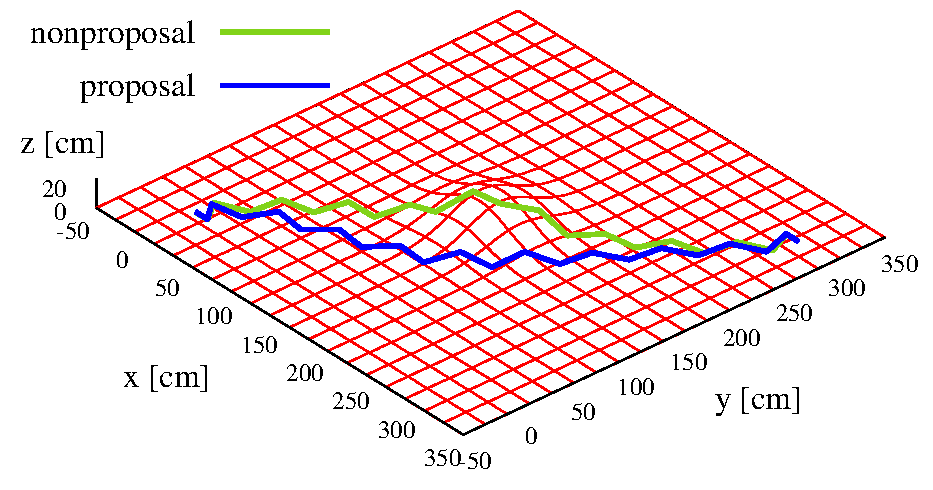
\includegraphics[width=\linewidth, clip]{./figure/sim_hrp2_hill_25_xyz.pdf}%
        \subcaption{$z_\mathrm{top} = 25.0\,\cm$}
        \label{fig:sim_hrp2_hill_25_xyz}%
    \end{subfigure}\\ %
    \vfil%
    \begin{subfigure}[c]{\linewidth}
        \centering%
        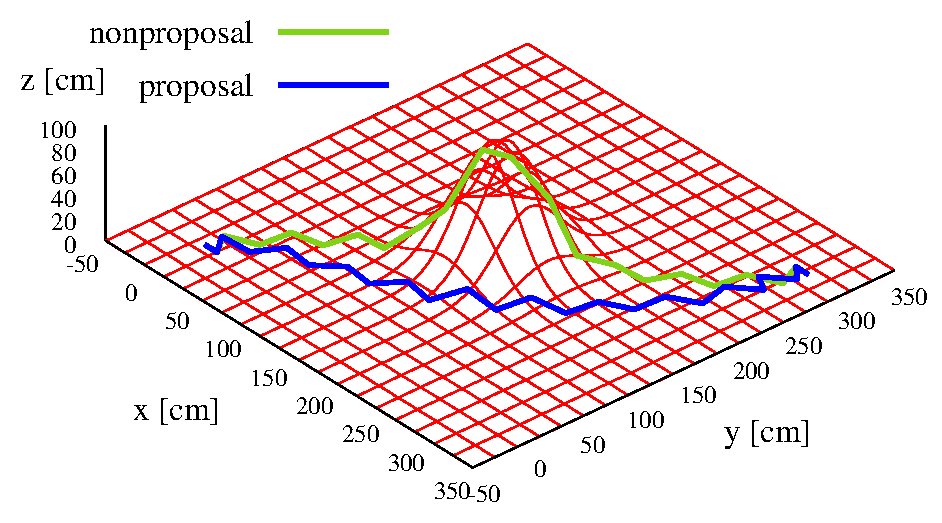
\includegraphics[width=\linewidth, clip]{./figure/sim_hrp2_hill_100_xyz.pdf}%
        \subcaption{$z_\mathrm{top} = 100.0\,\cm$}
        \label{fig:sim_hrp2_hill_100_xyz}%
    \end{subfigure}%
    \caption{Footsteps$x$-$y$-$z$view (single hill)}%
    \label{fig:sim_hrp2_hill}%
\end{figure}
\begin{figure}[pt]%
    \centering%
    \begin{subfigure}[c]{\linewidth}
        \centering%
        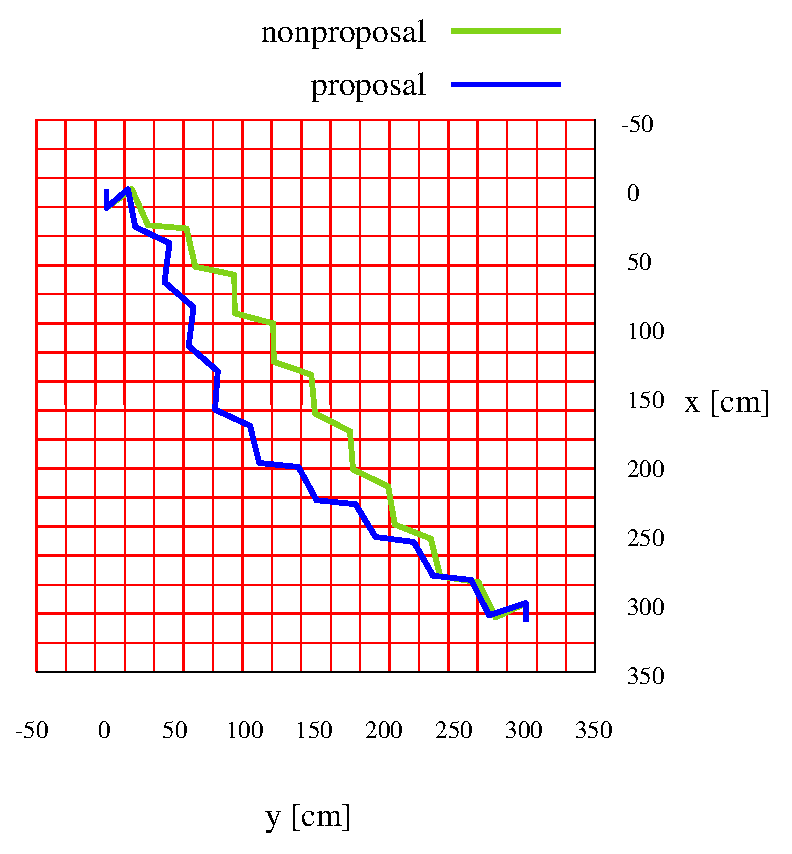
\includegraphics[width=0.55\linewidth, clip]{./figure/sim_hrp2_hill_25_xy.pdf}%
        \subcaption{$z_\mathrm{top} = 25.0\,\cm$}
        \label{fig:sim_hrp2_hill_25_xy}%
    \end{subfigure}\\ %
    \vfil%
    \begin{subfigure}[c]{\linewidth}
        \centering%
        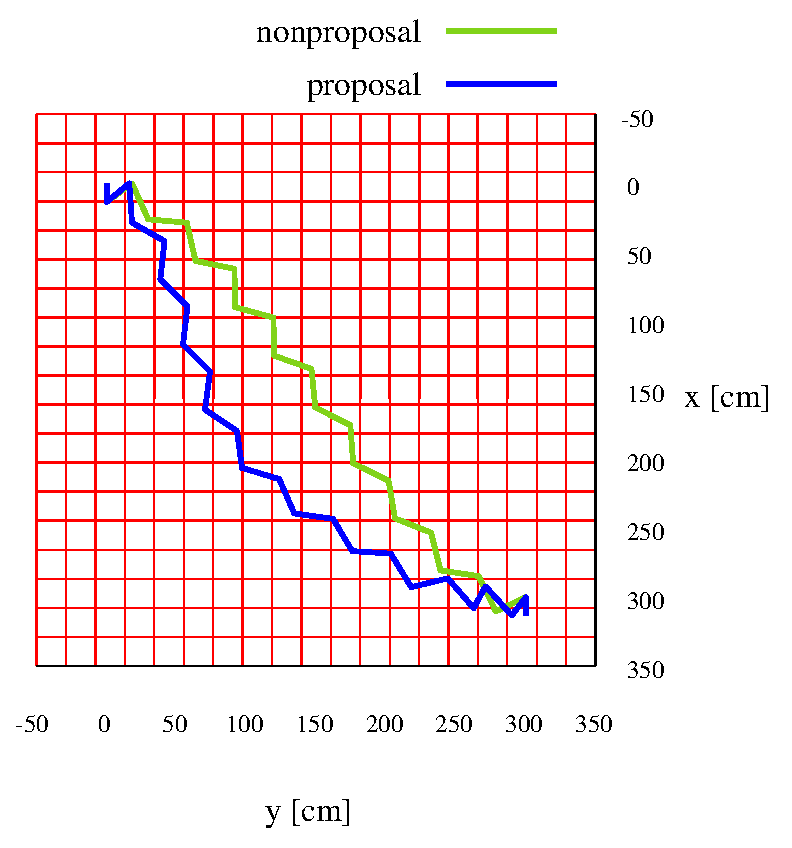
\includegraphics[width=0.55\linewidth, clip]{./figure/sim_hrp2_hill_100_xy.pdf}%
        \subcaption{$z_\mathrm{top} = 100.0\,\cm$}
        \label{fig:sim_hrp2_hill_100_xy}%
    \end{subfigure}%
    \caption{Footsteps$x$-$y$view (single hill)}%
    \label{fig:sim_hrp2_hill_xy}%
\end{figure}
\begin{figure}[pt]%
    \centering%
    \begin{subfigure}[c]{\linewidth}
        \centering%
        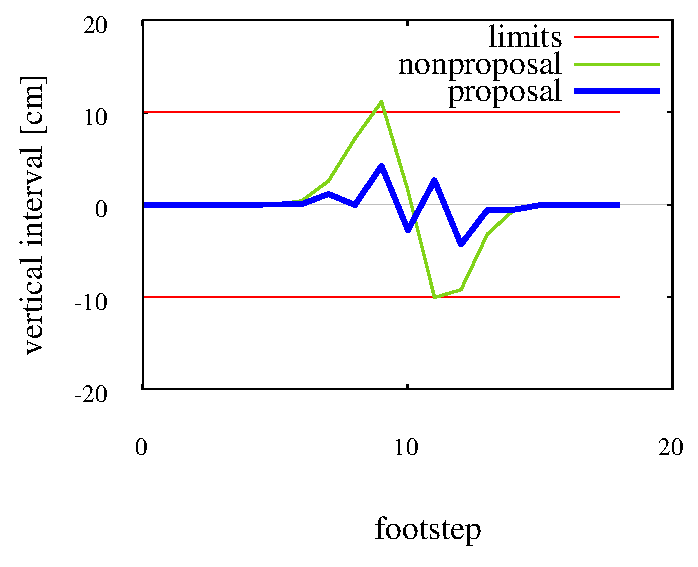
\includegraphics[width=0.75\linewidth, clip]{./figure/sim_hrp2_hill_25_zdiff.pdf}%
        \subcaption{$z_\mathrm{top} = 25.0\,\cm$}
        \label{fig:sim_hrp2_hill_25_zdiff}%
    \end{subfigure}\\ %
    \vfil%
    \begin{subfigure}[c]{\linewidth}
        \centering%
        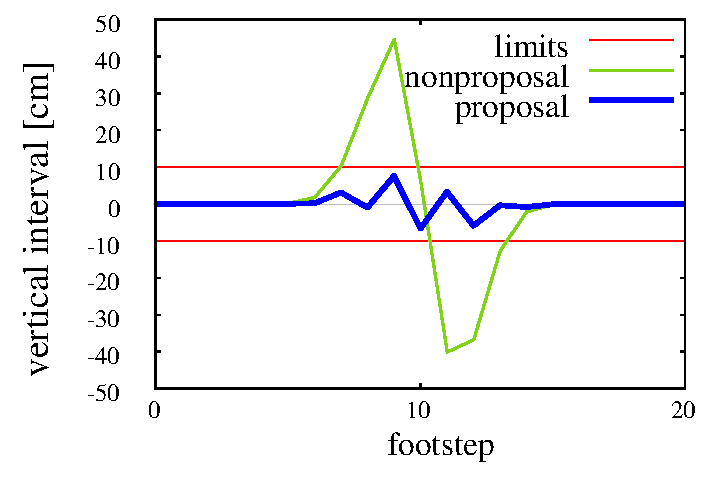
\includegraphics[width=0.75\linewidth, clip]{./figure/sim_hrp2_hill_100_zdiff.pdf}%
        \subcaption{$z_\mathrm{top} = 100.0\,\cm$}
        \label{fig:sim_hrp2_hill_100_zdiff}%
    \end{subfigure}%
    \caption{Vertical interval (single hill)}%
    \label{fig:sim_hrp2_hill_zdiff}%
\end{figure}
\begin{table}[pt]%
    \caption{Result of planning (single hill)}%
    \label{tab:sim_hrp2_hill}%
    \centering%
    \begin{tabular}{ccccc}%
        \toprule%
        $z_{\mathrm{top}}\,(\cm)$   &   $k_{\init}$ &   $k$     &   iteration   &   time$(\ms)$ \\%
        \midrule%
        plane                       &   $10$        &   $10$    &   $19$        &   $11.67$ \\%
        $25.0$                      &   $10$        &   $10$    &   $31$        &   $21.06$ \\%
        $100.0$                     &   $10$        &   $11$    &   $53$        &   $40.67$ \\%
        \bottomrule%
    \end{tabular}%
\end{table}

\subsection{二つの山を配置した場合}
次に,二つの山を配置した場合のシミュレーションを行った.
\begin{equation}
    \begin{aligned}
        z_{\field}\left( x ,\, y \right) & = z_{\mathrm{top}} \exp \left( - \frac{ \left( x - x_{c1} \right)^2 + \left( y - y_{c1} \right)^2}{2.0 \left( 30.0 \right)^2} \right) \\
                                         & = z_{\mathrm{top}} \exp \left( - \frac{ \left( x - x_{c2} \right)^2 + \left( y - y_{c2} \right)^2}{2.0 \left( 30.0 \right)^2} \right)
    \end{aligned}
\end{equation}
二つとも$z_{\mathrm{top}} = 100.0\,\cm$とし,
山の配置$(x_{c1} ,\, y_{c1})$,$(x_{c2} ,\, y_{c2})$を
$(75.0 ,\, 150.0)$,$(225.0 ,\, 0.0) (\cm)$とした場合と,
%$(75.0 ,\, 225.0)$,$(225.0 ,\, 75.0) (\cm)$とした場合,
$(75.0 ,\, 300.0)$,$(225.0 ,\, 150.0) (\cm)$とした場合の3パターンで計画を行った.

\Cref{fig:sim_hrp2_hill2},\cref{fig:sim_hrp2_hill2_xy},\cref{fig:sim_hrp2_hill2_zdiff},
\cref{tab:sim_hrp2_hill2}に計画結果を示す.
\Cref{fig:sim_hrp2_hill2_100_0_xyz},
\cref{fig:sim_hrp2_hill2_100_2_xyz}いずれにおいても
山の間を通って最短で目標へ到達する脚配置が計画されており,
\Cref{fig:sim_hrp2_hill2_100_0_zdiff},
\cref{fig:sim_hrp2_hill2_100_2_zdiff}を見ても
脚先の垂直移動は制約の範囲内に収まっていることから,
地形に合わせて最適な経路をとる脚配置が計画できていることがわかる.


\begin{figure}[pt]%
    \centering%
    \begin{subfigure}[c]{\linewidth}
        \centering%
        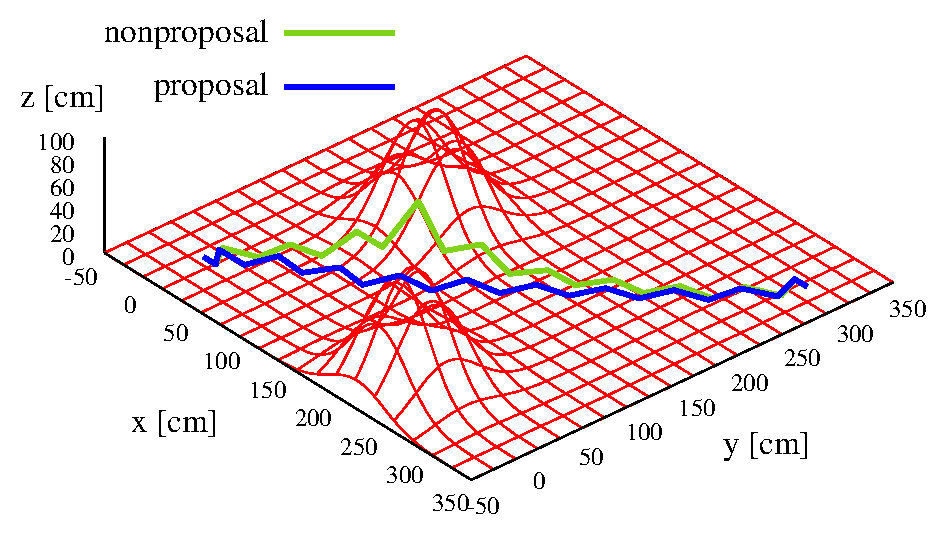
\includegraphics[width=\linewidth, clip]{./figure/sim_hrp2_hill2_100_0_xyz.pdf}%
        \subcaption{$(75.0 ,\, 150.0) ,\, (225.0 ,\, 0.0) (\cm)$}
        \label{fig:sim_hrp2_hill2_100_0_xyz}%
    \end{subfigure}\\ %
    % \begin{subfigure}[c]{\linewidth}
    %     \centering%
    %     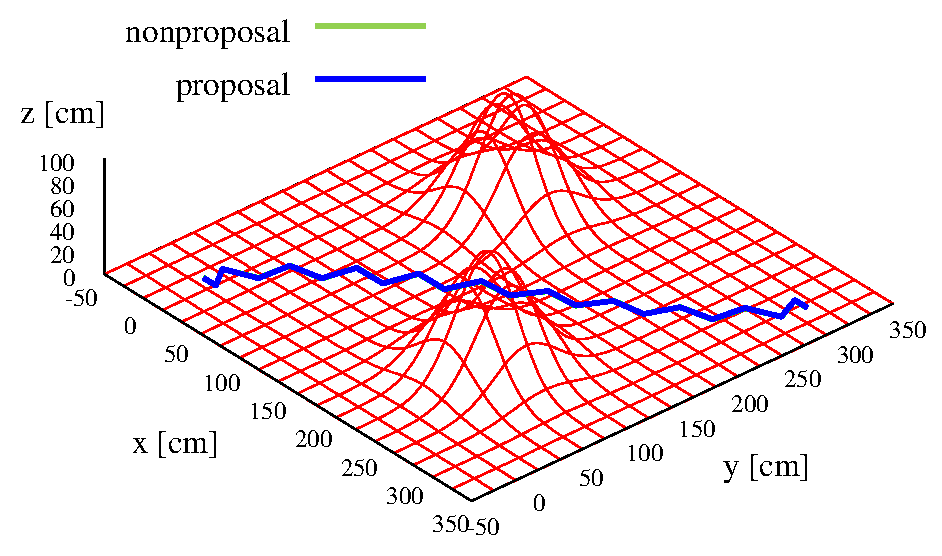
\includegraphics[width=\linewidth, clip]{./figure/sim_hrp2_hill2_100_1_xyz.pdf}%
    %     \subcaption{$(75.0 ,\, 225.0) ,\, (225.0 ,\, 75.0) (\cm)$}
    %     \label{fig:sim_hrp2_hill2_100_1_xyz}%
    % \end{subfigure}\\ %
    \begin{subfigure}[c]{\linewidth}
        \centering%
        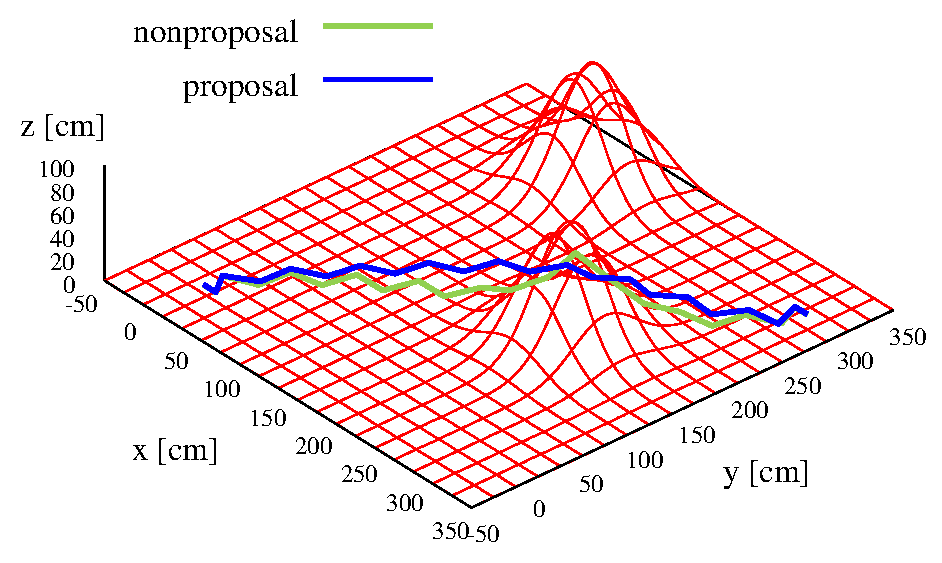
\includegraphics[width=\linewidth, clip]{./figure/sim_hrp2_hill2_100_2_xyz.pdf}%
        \subcaption{$(75.0 ,\, 300.0) ,\, (225.0 ,\, 150.0) (\cm)$}
        \label{fig:sim_hrp2_hill2_100_2_xyz}%
    \end{subfigure}%
    \caption{Footsteps$x$-$y$-$z$view (double hill)}%
    \label{fig:sim_hrp2_hill2}%
\end{figure}
\begin{figure}[pt]%
    \centering%
    \begin{subfigure}[c]{\linewidth}
        \centering%
        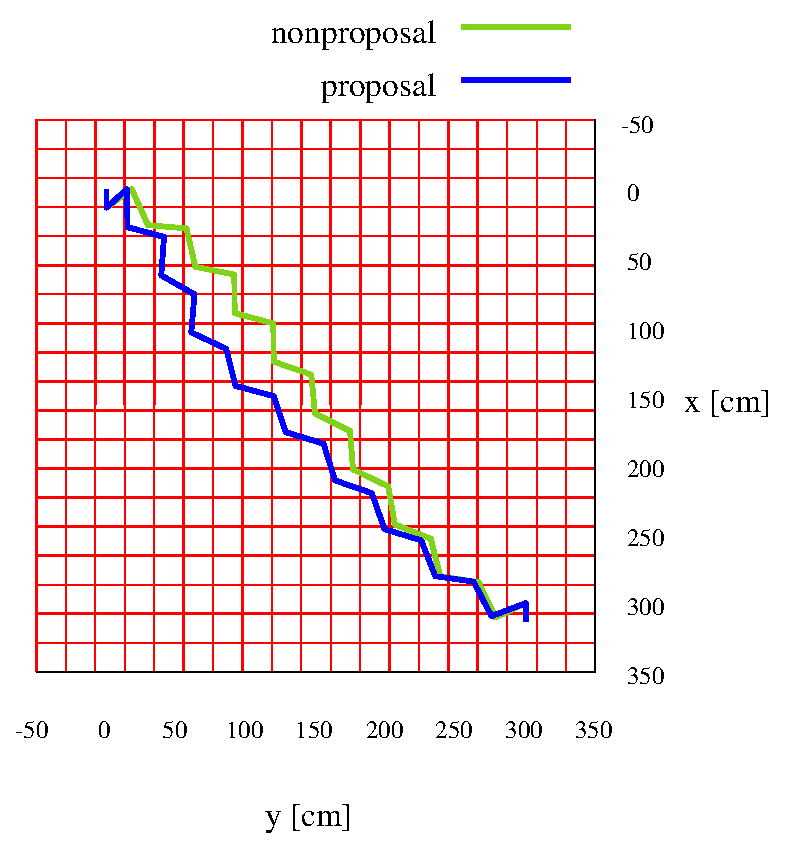
\includegraphics[width=0.55\linewidth, clip]{./figure/sim_hrp2_hill2_100_0_xy.pdf}%
        \subcaption{$(75.0 ,\, 150.0) ,\, (225.0 ,\, 0.0) (\cm)$}
        \label{fig:sim_hrp2_hill2_100_0_xy}%
    \end{subfigure}\\ %
    % \begin{subfigure}[c]{\linewidth}
    %     \centering%
    %     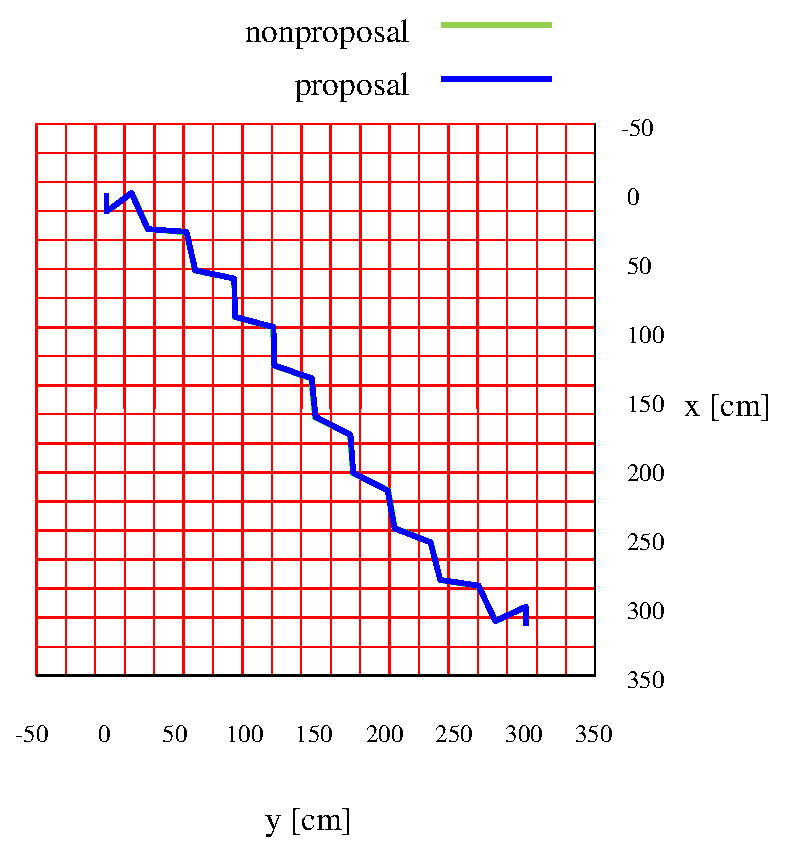
\includegraphics[width=0.55\linewidth, clip]{./figure/sim_hrp2_hill2_100_1_xy.pdf}%
    %     \subcaption{$(75.0 ,\, 225.0) ,\, (225.0 ,\, 75.0) (\cm)$}
    %     \label{fig:sim_hrp2_hill2_100_1_xy}%
    % \end{subfigure}\\ %
    \begin{subfigure}[c]{\linewidth}
        \centering%
        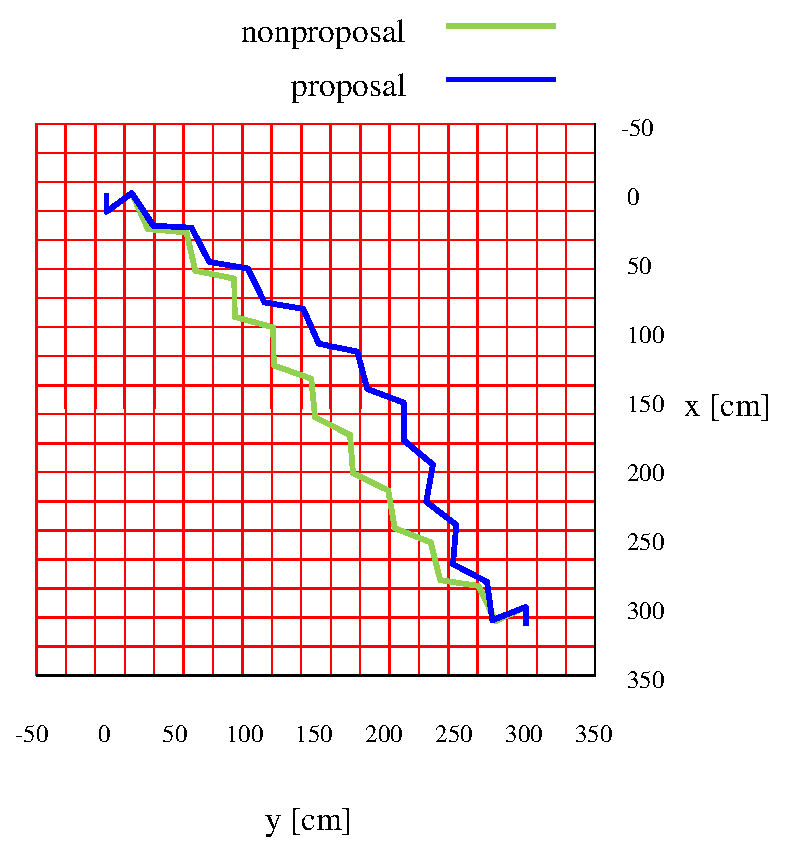
\includegraphics[width=0.55\linewidth, clip]{./figure/sim_hrp2_hill2_100_2_xy.pdf}%
        \subcaption{$(75.0 ,\, 300.0) ,\, (225.0 ,\, 150.0) (\cm)$}
        \label{fig:sim_hrp2_hill2_100_2_xy}%
    \end{subfigure}%
    \caption{Footsteps$x$-$y$view (double hill)}%
    \label{fig:sim_hrp2_hill2_xy}%
\end{figure}
\begin{figure}[pt]%
    \centering%
    \begin{subfigure}[c]{\linewidth}
        \centering%
        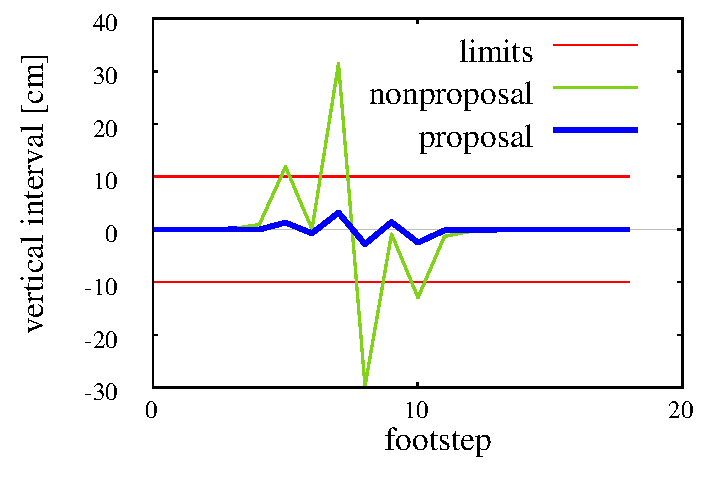
\includegraphics[width=0.75\linewidth, clip]{./figure/sim_hrp2_hill2_100_0_zdiff.pdf}%
        \subcaption{$(75.0 ,\, 150.0) ,\, (225.0 ,\, 0.0) (\cm)$}
        \label{fig:sim_hrp2_hill2_100_0_zdiff}%
    \end{subfigure}\\ %
    % \begin{subfigure}[c]{\linewidth}
    %     \centering%
    %     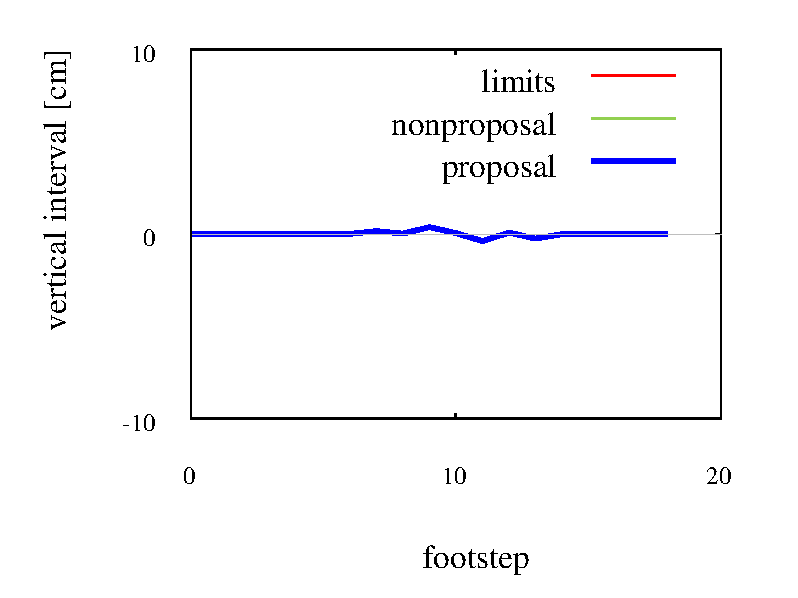
\includegraphics[width=0.75\linewidth, clip]{./figure/sim_hrp2_hill2_100_1_zdiff.pdf}%
    %     \subcaption{$(75.0 ,\, 225.0) ,\, (225.0 ,\, 75.0) (\cm)$}
    %     \label{fig:sim_hrp2_hill2_100_1_zdiff}%
    % \end{subfigure}\\ %
    \begin{subfigure}[c]{\linewidth}
        \centering%
        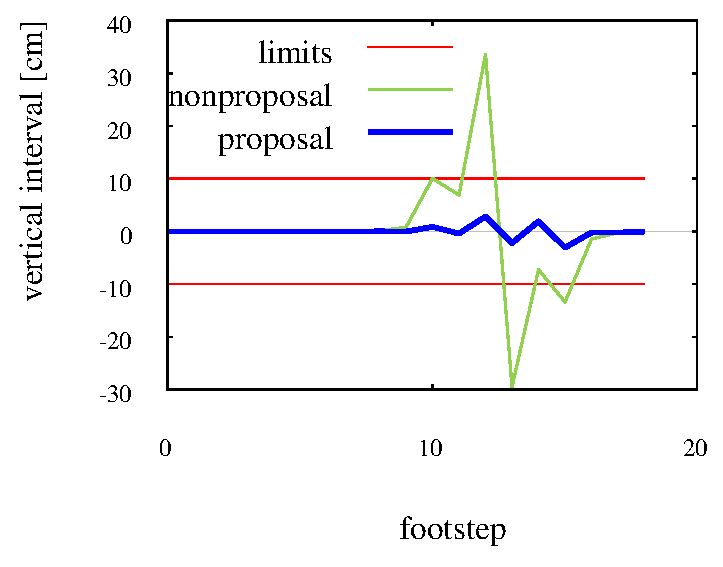
\includegraphics[width=0.75\linewidth, clip]{./figure/sim_hrp2_hill2_100_2_zdiff.pdf}%
        \subcaption{$(75.0 ,\, 300.0) ,\, (225.0 ,\, 150.0) (\cm)$}
        \label{fig:sim_hrp2_hill2_100_2_zdiff}%
    \end{subfigure}%
    \caption{Vertical interval (double hill)}%
    \label{fig:sim_hrp2_hill2_zdiff}%
\end{figure}
\begin{table}[t]%
    \caption{Result of planning (double hill)}%
    \label{tab:sim_hrp2_hill2}%
    \centering%
    \begin{tabular}{ccccc}%
        \toprule%
        $(x_c ,\, y_c)\,(\cm)$                                      &   $k_{\init}$ &   $k$     &   iteration   &   time$(\ms)$ \\%
        \midrule%
        plane                                                       &   $10$        &   $10$    &   $19$        &   $11.67$ \\%
        $(75.0 ,\, 150.0) ,\, (225.0 ,\, \phantom{00}0.0) (\cm)$    &   $10$        &   $10$    &   $22$        &   $14.28$ \\%
        % $(75.0 ,\, 225.0) ,\, (225.0 ,\, \phantom{0}75.0) (\cm)$    &   $10$        &   $10$    &   $19$        &   $12.09$ \\%
        $(75.0 ,\, 300.0) ,\, (225.0 ,\, 150.0) (\cm)$              &   $10$        &   $10$    &   $22$        &   $14.19$ \\%
        \bottomrule%
    \end{tabular}%
\end{table}

\subsection{スロープ型の地形でのシミュレーション}
\label{subsec:sim_hrp2_lope}
初期状態$\bm{q}^0 = ( 0.0 ,\, 0.0 ,\, 0.0 ,\, 13.5 ,\, 0.0 ,\, 0.0 )^T\,(\cm ,\, \degrm)$から
目標状態$\bm{q}_{\goal} = ( 150.0 ,\, 450.0 ,\, 0.0 ,\, 13.5 ,\, 0.0 ,\, 0.0 )^T$へと向かう計画を行う.
地形としては,$y$軸方向において平面と傾斜角$\theta_{\slope}$の斜面が$y = 100\,\cm$の位置で接続しているスロープ型の地形を用いる.
スロープは$y = 100\,\cm$の位置で終了し,平面形状へと戻る.
\begin{equation}
    z_{\field}\left( x ,\, y \right) =
        \begin{cases}
            0.0                                           & \left( y < 100.0 \right) \\
            \left( y - 100.0 \right) \tan \theta_{\slope} & \left( 100.0 \leq y < 350.0 \right) \\
            250.0 \tan \theta_{\slope}                    & \left( 350.0 \leq y \right)
        \end{cases}
\end{equation}
$\theta = 5.0\degree$で計画を行う.

\begin{figure}[pt]%
    \centering%
    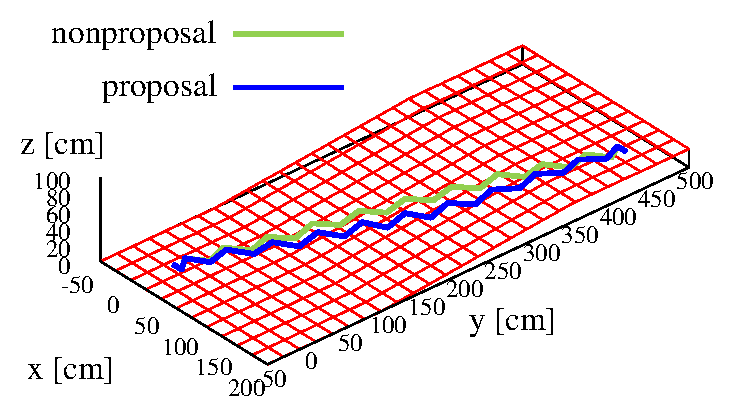
\includegraphics[width=0.9\linewidth, clip]{./figure/sim_hrp2_slope_50_xyz.pdf}%
    \caption{Footsteps x-y-z view (slope)}%
    \label{fig:sim_hrp2_slope}%
\end{figure}
\begin{figure}[pt]%
    \centering%
    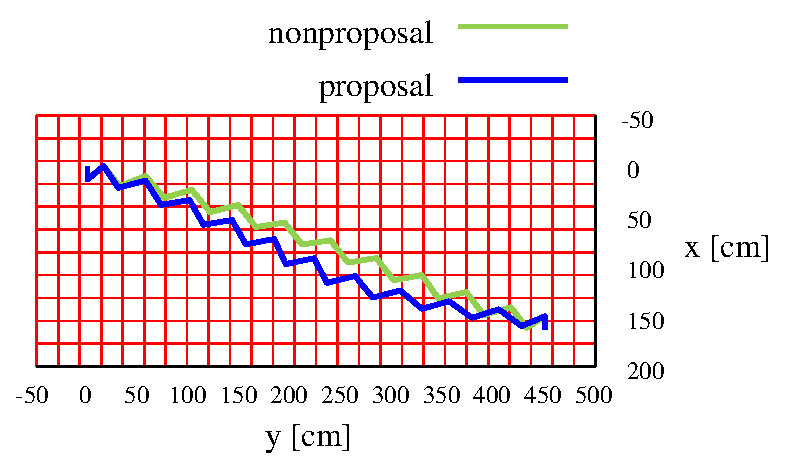
\includegraphics[width=0.8\linewidth, clip]{./figure/sim_hrp2_slope_50_xy.pdf}%
    \caption{Footsteps x-y view (slope)}%
    \label{fig:sim_hrp2_slope_xy}%
\end{figure}
\begin{figure}[pt]%
    \centering%
    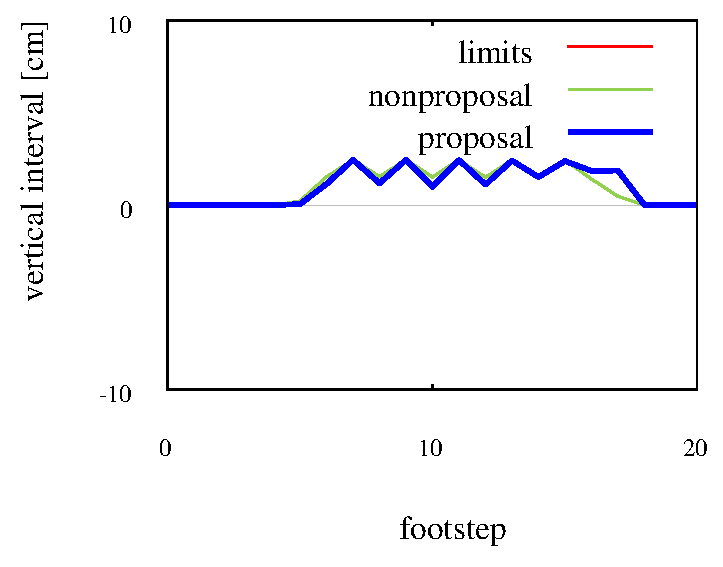
\includegraphics[width=0.7\linewidth, clip]{./figure/sim_hrp2_slope_50_zdiff.pdf}%
    \caption{Vertical interval (slope)}%
    \label{fig:sim_hrp2_slope_zdiff}%
\end{figure}
\begin{table}[t]%
    \caption{Result of planning (slope)}%
    \label{tab:sim_hrp2_slope}%
    \centering%
    \begin{tabular}{ccccc}%
        \toprule%
        $\theta_{\slope}\,(\degrm)$ &   $k_{\init}$ &   $k$     &   iteration   &   time$(\ms)$ \\%
        \midrule%
        plane                       &   $11$        &   $11$    &   $14$        &   $7.45$ \\%
        $5.0$                       &   $11$        &   $11$    &   $20$        &   $14.11$ \\%
        \bottomrule%
    \end{tabular}
\end{table}
\Cref{fig:sim_hrp2_slope},\cref{fig:sim_hrp2_slope_xy},\cref{fig:sim_hrp2_slope_zdiff},
\cref{tab:sim_hrp2_slope}に計画結果を示す.
地形を考慮しない場合でも地形適応制約を破らない範囲であるため,脚配置や計算時間,反復回数などに大きな差はない.
提案手法においては反復計算の過程で垂直移動の仮想的な入力の最小化評価が行われているため,
平面上での計画と比較すると若干経路が変化している.
この結果から,水平方向の動作に加えて垂直方向の動作も正しく評価され,最適化されていることがわかる.


\subsection{計算時間の評価}
適用する二足歩行ロボットの一歩進むのにかかる時間よりも計算時間が十分に短ければ,
オンラインでの再計画が可能となり,実時間性がある.
今回シミュレーションした地形においては,
いずれの結果においても実機HRP-2の歩行周期全体のみならず,
両脚支持期間よりも短い時間で計画できており,
連続的変化のある地形においては実時間性があることが示された.




\section{不連続な変化のある地形上での計画}
\begin{table}[t]%
    \centering
    % \small
    \caption{Map parameters for HRP-2 (discontinuous field)}
    \label{tab:sim_hrp2_param_map_discon}
    \begin{tabular}{cc}
        \toprule
        parameters              &   value \\
        \midrule
        $D_\mathrm{grid}$       &   $1.0\,\cm$ \\
        $D_\mathrm{sample}$     &   $0.2\,\cm$ \\
        \bottomrule
    \end{tabular}
\end{table}

不連続な変化のある地形として,段差のある地形と階段状の地形を考えることとし,
それらの地形上での計画結果を確認する.
なお,地形構築の際のグリッドマップのサイズと関数からのサンプリング間隔は,
不連続な変化がある部分に対応するセルが小さくなるよう,
\cref{tab:sim_hrp2_param_map_discon}に示す通りそれぞれ$1.0\,\cm$,$0.2\,\cm$とする.
段差や階段のような変化が含まれるセルでは,領域内のサンプル点の平均をとったときに
実際の地形には存在しない,段と段との間の中途半端な値が表現されてしまうことになる.
現在の地形適応の方法および地形情報構築方法ではこれは避けられないため,
できるだけグリッドサイズを小さくすることでこれに対応することとする.

% \subsection{段差のある地形}
% \begin{figure}[pt]%
%     \centering%
%     \begin{subfigure}[c]{\linewidth}
%         \centering%
%         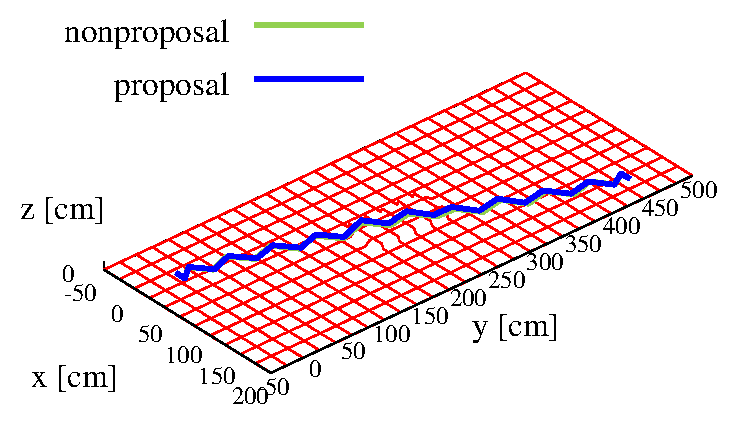
\includegraphics[width=\linewidth, clip]{./figure/sim_hrp2_uneven_50_xyz.pdf}%
%         \subcaption{$z_\mathrm{top} = 25.0\,\cm$}
%         \label{fig:sim_hrp2_uneven_50_xyz}%
%     \end{subfigure}\\ %
%     \vfil%
%     \begin{subfigure}[c]{\linewidth}
%         \centering%
%         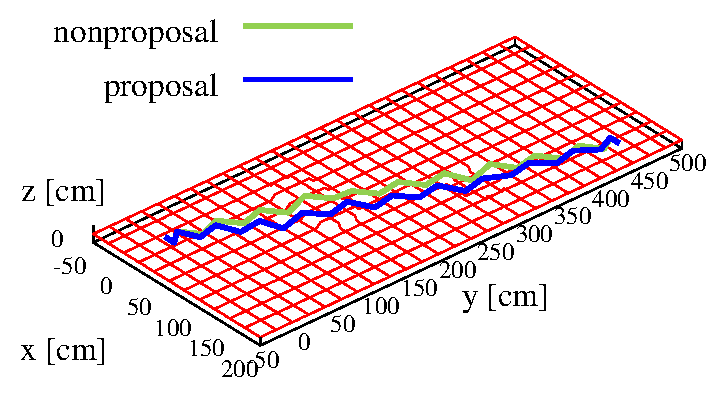
\includegraphics[width=\linewidth, clip]{./figure/sim_hrp2_uneven2_50_-50_xyz.pdf}%
%         \subcaption{$z_\mathrm{top} = 100.0\,\cm$}
%         \label{fig:sim_hrp2_uneven2_50_-50_xyz}%
%     \end{subfigure}%
%     \caption{Footsteps$x$-$y$-$z$view (single uneven)}%
%     \label{fig:sim_hrp2_uneven}%
% \end{figure}
% \begin{figure}[pt]%
%     \centering%
%     \begin{subfigure}[c]{\linewidth}
%         \centering%
%         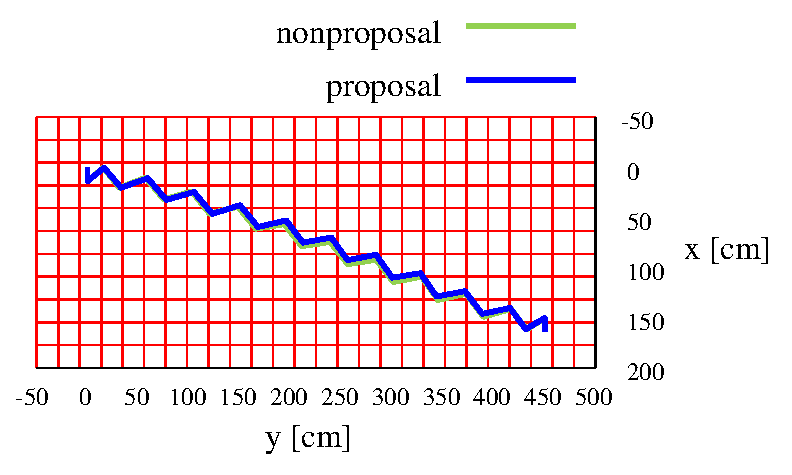
\includegraphics[width=0.55\linewidth, clip]{./figure/sim_hrp2_uneven_50_xy.pdf}%
%         \subcaption{$z_\mathrm{top} = 25.0\,\cm$}
%         \label{fig:sim_hrp2_uneven_50_xy}%
%     \end{subfigure}\\ %
%     \vfil%
%     \begin{subfigure}[c]{\linewidth}
%         \centering%
%         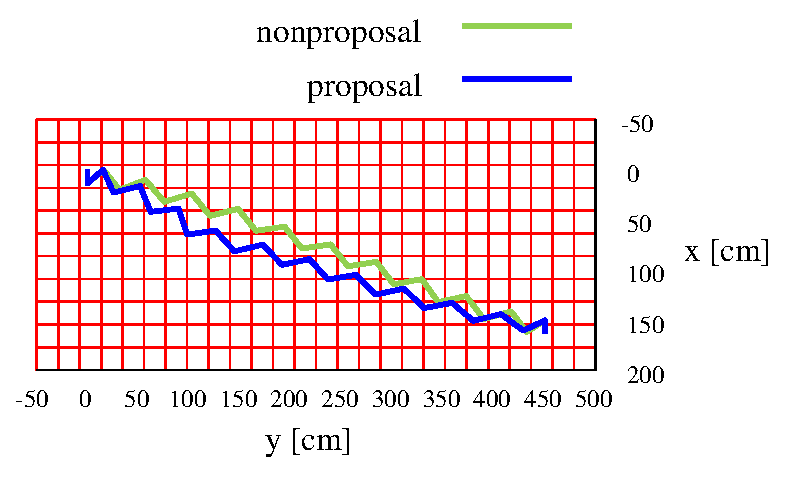
\includegraphics[width=0.55\linewidth, clip]{./figure/sim_hrp2_uneven2_50_-50_xy.pdf}%
%         \subcaption{$z_\mathrm{top} = 100.0\,\cm$}
%         \label{fig:sim_hrp2_uneven2_50_-50_xy}%
%     \end{subfigure}%
%     \caption{Footsteps$x$-$y$view (single uneven)}%
%     \label{fig:sim_hrp2_uneven_xy}%
% \end{figure}
% \begin{figure}[pt]%
%     \centering%
%     \begin{subfigure}[c]{\linewidth}
%         \centering%
%         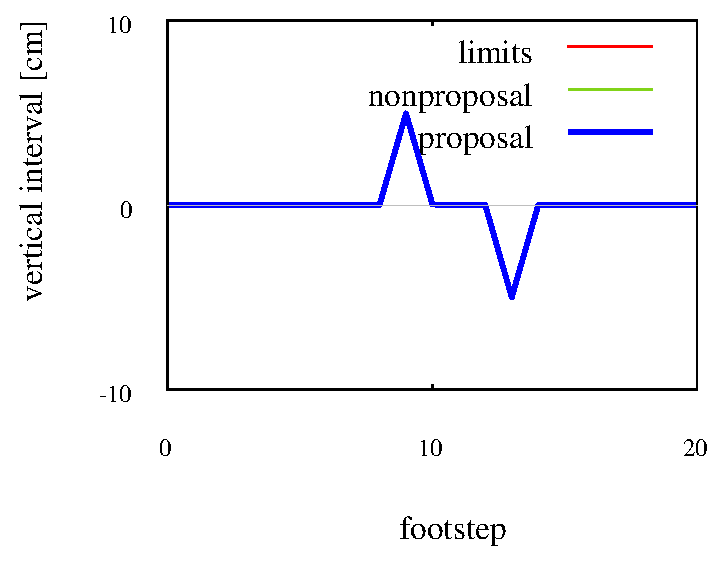
\includegraphics[width=0.75\linewidth, clip]{./figure/sim_hrp2_uneven_50_zdiff.pdf}%
%         \subcaption{$z_\mathrm{top} = 25.0\,\cm$}
%         \label{fig:sim_hrp2_uneven_50_zdiff}%
%     \end{subfigure}\\ %
%     \vfil%
%     \begin{subfigure}[c]{\linewidth}
%         \centering%
%         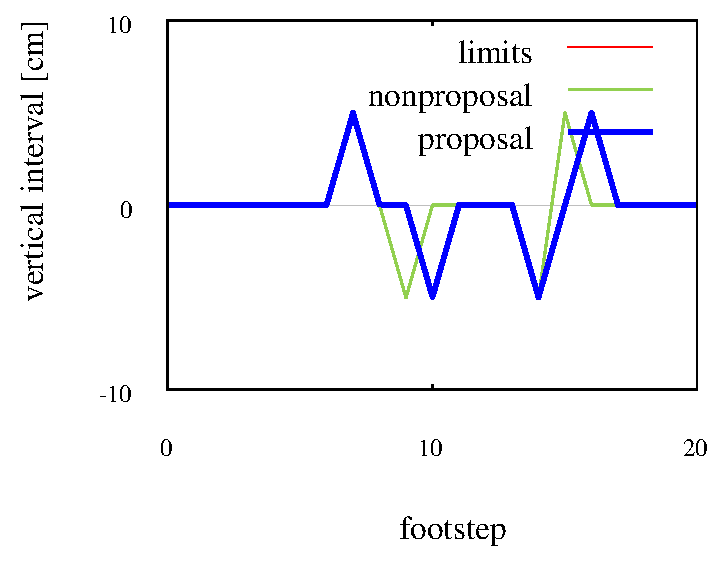
\includegraphics[width=0.75\linewidth, clip]{./figure/sim_hrp2_uneven2_50_-50_zdiff.pdf}%
%         \subcaption{$z_\mathrm{top} = 100.0\,\cm$}
%         \label{fig:sim_hrp2_uneven2_50_-50_zdiff}%
%     \end{subfigure}%
%     \caption{Vertical interval (single uneven)}%
%     \label{fig:sim_hrp2_uneven_zdiff}%
% \end{figure}
% \begin{table}[pt]%
%     \caption{Result of planning (single hill)}%
%     \label{tab:sim_hrp2_uneven}%
%     \centering%
%     \begin{tabular}{ccccc}%
%         \toprule%
%        $z_{\mathrm{top}}\,(\cm)$&$k_{\init}$&$k$ & iteration & time$(\ms)$ \\%
%         \midrule%
%         plane                     &$10$       &$10$&$19$     &$11.67$ \\%
%        $25.0$                   &$10$       &$10$&$31$     &$21.06$ \\%
%        $100.0$                  &$10$       &$11$&$53$     &$40.67$ \\%
%         \bottomrule%
%     \end{tabular}%
% \end{table}

\subsection{上り階段地形}
初期状態$\bm{q}^0 = ( 0.0 ,\, 0.0 ,\, 0.0 ,\, 13.5 ,\, 0.0 ,\, 0.0 )^T\,(\cm ,\, \degrm)$から
目標状態$\bm{q}_{\goal} = ( 0.0 ,\, 250.0 ,\, 0.0 ,\, 13.5 ,\, 0.0 ,\, 0.0 )^T$へと向かう計画を行う.
地形としては,$yy = 50.0\,\cm$から始まり$y$方向へ$25.0\,\cm$進むごとに$8.0\,\cm$ずつ上る5段の上り階段とする.
\begin{equation}
    z_{\field}\left( x ,\, y \right) =
        \begin{cases}
            \phantom{0}0.0  &   \left( y < 50.0 \right) \\
            \phantom{0}8.0  &   \left( 50.0  \leq y  < 75.0 \right) \\
            16.0            &   \left( 45.0  \leq y < 100.0 \right) \\
            24.0            &   \left( 100.0 \leq y < 125.0 \right) \\
            32.0            &   \left( 125.0 \leq y < 150.0 \right) \\
            40.0            &   \left( 150.0 \leq y \right)
        \end{cases}
\end{equation}
また,それを半歩$d_{xy \mathrm{xy}} / 4 = 12.5\,\cm$だけ前方にずらした地形でも計画を行う.
\begin{equation}
    z_{\field}\left( x ,\, y \right) =
        \begin{cases}
            \phantom{0}0.0  &   \left( y < 62.5 \right) \\
            \phantom{0}8.0  &   \left( 62.5  \leq y  < 87.5 \right) \\
            16.0            &   \left( 87.5  \leq y < 112.5 \right) \\
            24.0            &   \left( 112.5 \leq y < 137.5 \right) \\
            32.0            &   \left( 137.5 \leq y < 162.5 \right) \\
            40.0            &   \left( 162.5 \leq y \right)
        \end{cases}
\end{equation}

\Cref{fig:sim_hrp2_stair_up},\cref{fig:sim_hrp2_stair_up_xy},\cref{fig:sim_hrp2_stair_up_zdiff},
\cref{tab:sim_hrp2_stair_up}に計画結果を示す.
2パターンの配置のうち,前者では初期位置付近で余計に歩行し,
同じ段に二歩の間留まるといった挙動を含む計画となっている.
これは,現在の解法は不連続な制約条件の変化に弱く求解性能が落ちるため,
反復計算の初期で局所解に陥っているためである.
しかし,わずかに地形の変化した後者においては
初期ステップ数$6$のまま$14$回の反復で解に収束していること,
またいずれの計画も両脚支持期間以下の時間で計算を終えられていることから,
最適化計算手法の修正や変更で改善できると考えられる.

\begin{figure}[pt]%
    \centering%
    \begin{subfigure}[c]{\linewidth}
        \centering%
        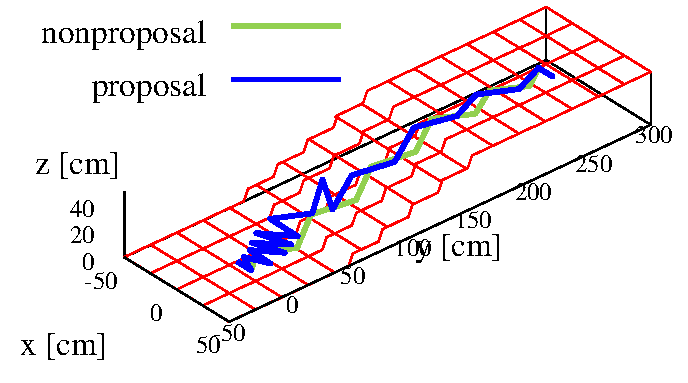
\includegraphics[width=0.9\linewidth, clip]{./figure/sim_hrp2_stair_upbad_xyz.pdf}%
        \subcaption{Reference placement}
        \label{fig:sim_hrp2_stair_upbad_xyz}%
    \end{subfigure}\\ %
    \vfil%
    \begin{subfigure}[c]{\linewidth}
        \centering%
        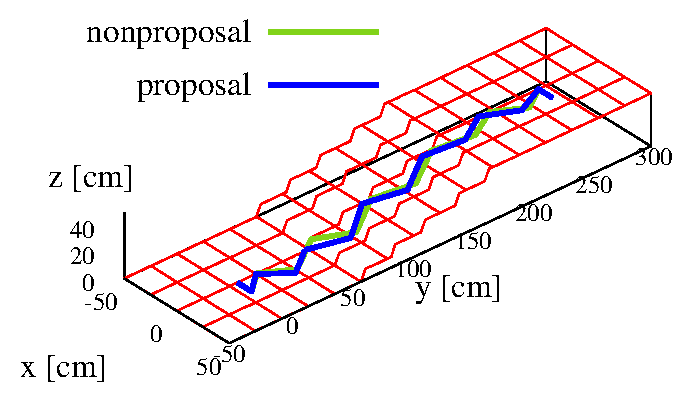
\includegraphics[width=0.9\linewidth, clip]{./figure/sim_hrp2_stair_up_xyz.pdf}%
        \subcaption{Placement to a half step length forward}
        \label{fig:sim_hrp2_stair_upgood_xyz}%
    \end{subfigure}%
    \caption{Footsteps$x$-$y$-$z$view (upward stairway)}%
    \label{fig:sim_hrp2_stair_up}%
\end{figure}
\begin{figure}[pt]%
    \centering%
    \begin{subfigure}[c]{\linewidth}
        \centering%
        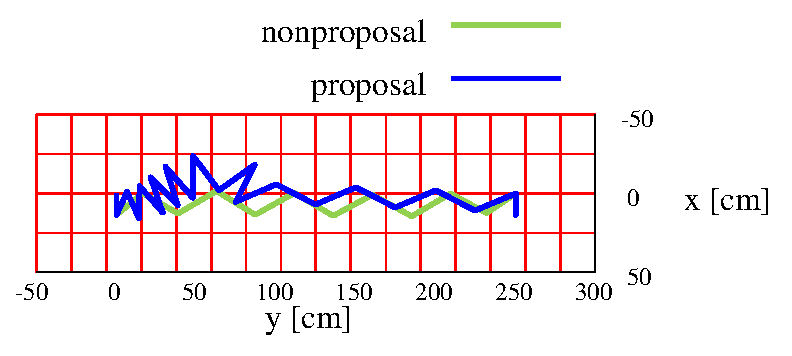
\includegraphics[width=0.9\linewidth, clip]{./figure/sim_hrp2_stair_upbad_xy.pdf}%
        \subcaption{Reference placement}
        \label{fig:sim_hrp2_stair_upbad_xy}%
    \end{subfigure}\\ %
    \vspace{25truemm}%
    \begin{subfigure}[c]{\linewidth}
        \centering%
        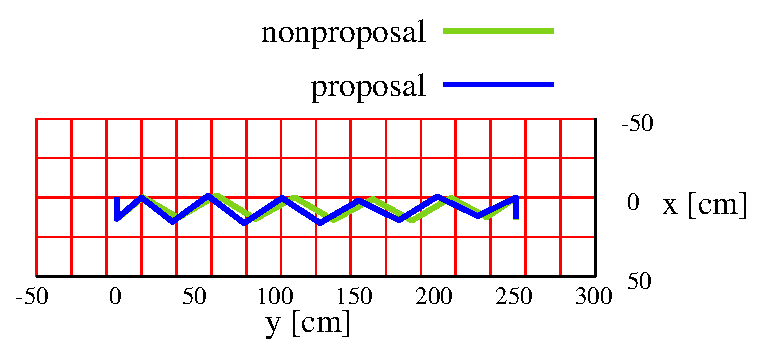
\includegraphics[width=0.9\linewidth, clip]{./figure/sim_hrp2_stair_up_xy.pdf}%
        \subcaption{Placement to a half step length forward}
        \label{fig:sim_hrp2_stair_upgood_xy}%
    \end{subfigure}%
    \caption{Footsteps$x$-$y$view (upward stairway)}%
    \label{fig:sim_hrp2_stair_up_xy}%
\end{figure}
\begin{figure}[pt]%
    \centering%
    \begin{subfigure}[c]{\linewidth}
        \centering%
        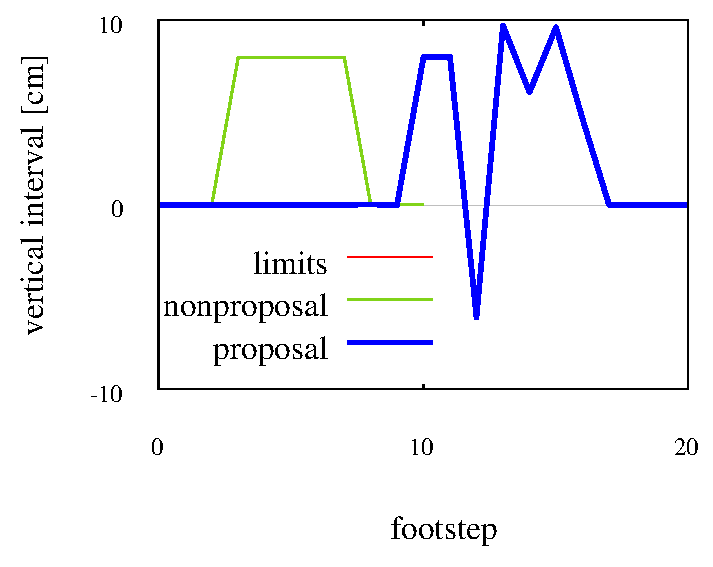
\includegraphics[width=0.75\linewidth, clip]{./figure/sim_hrp2_stair_upbad_zdiff.pdf}%
        \subcaption{Reference placement}
        \label{fig:sim_hrp2_stair_upbad_zdiff}%
    \end{subfigure}\\ %
    \vfil%
    \begin{subfigure}[c]{\linewidth}
        \centering%
        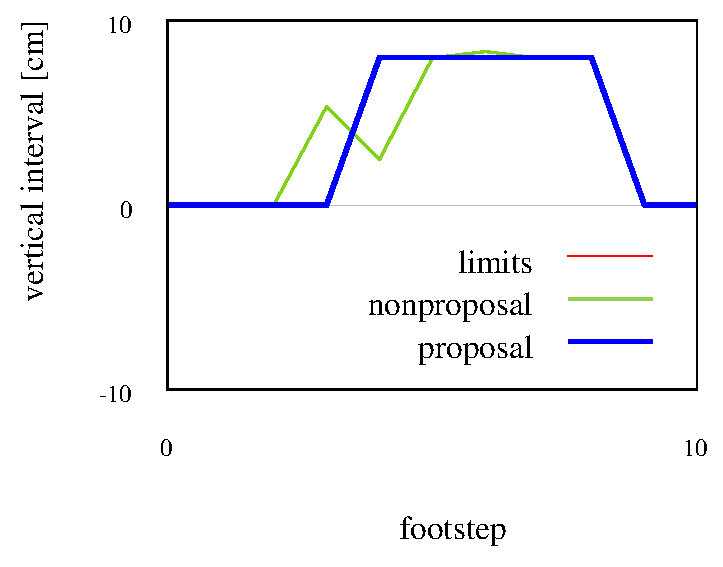
\includegraphics[width=0.75\linewidth, clip]{./figure/sim_hrp2_stair_up_zdiff.pdf}%
        \subcaption{Placement to a half step length forward}
        \label{fig:sim_hrp2_stair_upgood_zdiff}%
    \end{subfigure}%
    \caption{Vertical interval (upward stairway)}%
    \label{fig:sim_hrp2_stair_up_zdiff}%
\end{figure}
\begin{table}[pt]%
    \caption{Result of planning (upward stairway)}%
    \label{tab:sim_hrp2_stair_up}%
    \centering%
    \begin{tabular}{ccccc}%
        \toprule%
                            &   $k_{\init}$ &   $k$     &   iteration   &   time$(\ms)$ \\%
        \midrule%
        plane               &   $6$         &   $6$     &   $12$        &   $1.85$ \\%
        reference           &   $6$         &   $11$    &   $164$       &   $59.63$ \\%
        half step forward   &   $6$         &   $6$     &   $14$        &   $2.11$ \\%
        \bottomrule%
    \end{tabular}%
\end{table}

また,\cref{fig:sim_hrp2_stair_upbad_zdiff}を見ると,
両脚間の高低差は$8.0$であることが理想であるが
異なる値をとっていることがわかる.
これは,グリッドマップ上で不連続な変化をしている段差付近のセルを踏み,
地形形状を表現する補間関数が本来の形状にない値を返してしまうためである.
この問題に対しては,脚先の三次元姿勢をモデルとして考慮し,
これに対して制限制約をかけることで解決できると考えられる.
三次元姿勢を考慮することで,不連続な変化のある地形付近の,
補間関数の傾きが急峻となる領域を回避するような計画となると考えられるためである.


\subsection{下り階段地形}
初期状態$\bm{q}^0 = ( 0.0 ,\, 0.0 ,\, 0.0 ,\, 13.5 ,\, 0.0 ,\, 0.0 )^T\,(\cm ,\, \degrm)$から
目標状態$\bm{q}_{\goal} = ( 0.0 ,\, 250.0 ,\, 0.0 ,\, 13.5 ,\, 0.0 ,\, 0.0 )^T$へと向かう計画を行う.
地形としては,$yy = 50.0\,\cm$から始まり$y$方向へ$25.0\,\cm$進むごとに$8.0\,\cm$ずつ下る5段の下り階段とする.
\begin{equation}
    z_{\field}\left( x ,\, y \right) =
        \begin{cases}
            40.0            &   \left( y < 50.0 \right) \\
            32.0            &   \left( 50.0  \leq y  < 75.0 \right) \\
            24.0            &   \left( 75.0  \leq y < 100.0 \right) \\
            16.0            &   \left( 100.0 \leq y < 125.0 \right) \\
            \phantom{0}8.0  &   \left( 125.0 \leq y < 150.0 \right) \\
            \phantom{0}0.0  &   \left( 150.0 \leq y \right)
        \end{cases}
\end{equation}
また,それを半歩$d_{xy \mathrm{xy}} / 4 = 12.5\,\cm$だけ前方にずらした地形でも計画を行う.
\begin{equation}
    z_{\field}\left( x ,\, y \right) =
        \begin{cases}
            40.0            &   \left( y < 62.5 \right) \\
            32.0            &   \left( 62.5  \leq y  < 87.5 \right) \\
            24.0            &   \left( 87.5  \leq y < 112.5 \right) \\
            16.0            &   \left( 112.5 \leq y < 137.5 \right) \\
            \phantom{0}8.0  &   \left( 137.5 \leq y < 162.5 \right) \\
            \phantom{0}0.0  &   \left( 162.5 \leq y \right)
        \end{cases}
\end{equation}

\Cref{fig:sim_hrp2_stair_down},\cref{fig:sim_hrp2_stair_down_xy},\cref{fig:sim_hrp2_stair_down_zdiff},
\cref{tab:sim_hrp2_stair_down}に計画結果を示す.
上り階段地形と同様に,半歩分の配置の違いで結果に差が出ており,
不連続な変化の地形に対しては計算が不安定となり求解性能が低下していることがわかる.

\subsection{計算時間についての評価}
不連続な地形に対しては計算が不安定化してしまうことが明らかとなったが,
いずれの結果においても計算自体は両足支持期間よりも短く,実時間性は保たれている.
これは,計画アルゴリズムにおける収束見込み判定とステップ数の増補により,
問題が再定義されたことで局所解から脱することができたためである.

\begin{figure}[pt]%
    \centering%
    \begin{subfigure}[c]{\linewidth}
        \centering%
        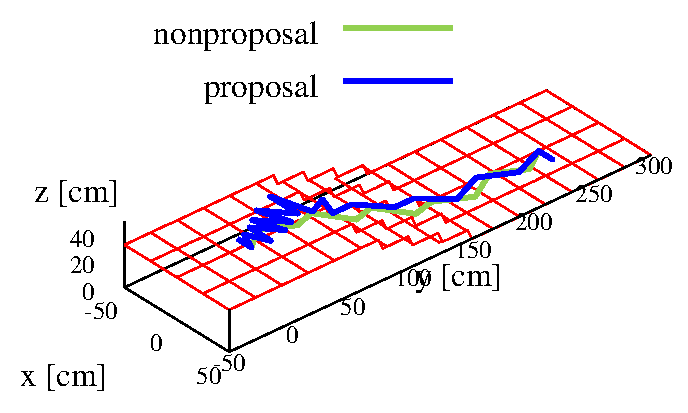
\includegraphics[width=0.9\linewidth, clip]{./figure/sim_hrp2_stair_downbad_xyz.pdf}%
        \subcaption{Reference placement}
        \label{fig:sim_hrp2_stair_downbad_xyz}%
    \end{subfigure}\\ %
    \vfil%
    \begin{subfigure}[c]{\linewidth}
        \centering%
        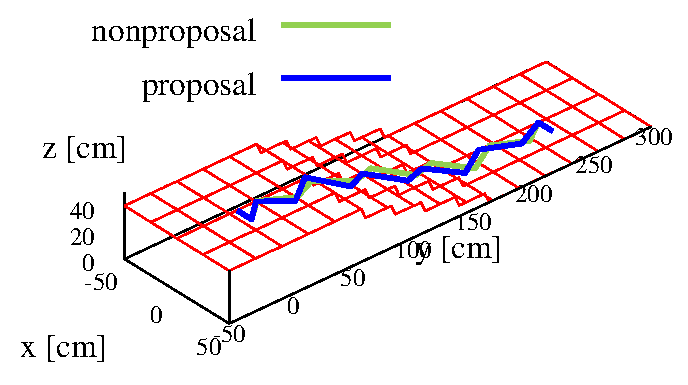
\includegraphics[width=0.9\linewidth, clip]{./figure/sim_hrp2_stair_down_xyz.pdf}%
        \subcaption{Placement to a half step length forward}
        \label{fig:sim_hrp2_stair_downgood_xyz}%
    \end{subfigure}%
    \caption{Footsteps$x$-$y$-$z$view (downward stairway)}%
    \label{fig:sim_hrp2_stair_down}%
\end{figure}
\begin{figure}[pt]%
    \centering%
    \begin{subfigure}[c]{\linewidth}
        \centering%
        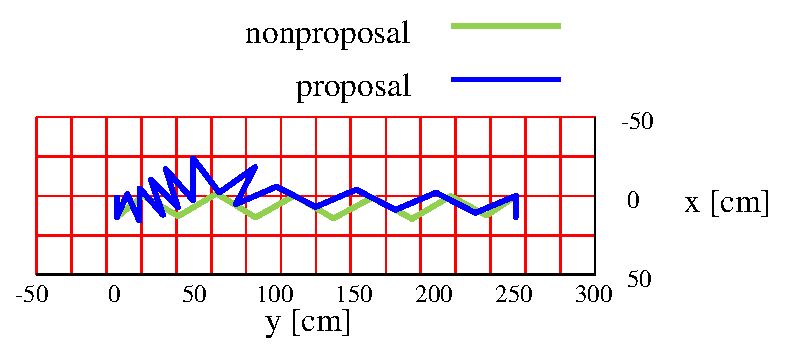
\includegraphics[width=0.9\linewidth, clip]{./figure/sim_hrp2_stair_downbad_xy.pdf}%
        \subcaption{Reference placement}
        \label{fig:sim_hrp2_stair_downbad_xy}%
    \end{subfigure}\\ %
    \vspace{10truemm}%
    \begin{subfigure}[c]{\linewidth}
        \centering%
        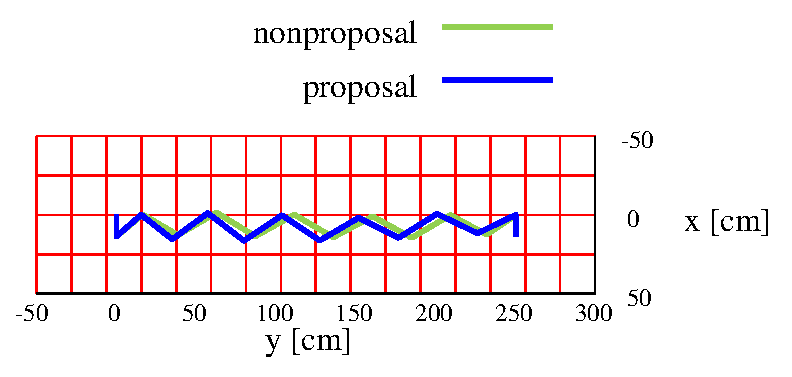
\includegraphics[width=0.9\linewidth, clip]{./figure/sim_hrp2_stair_down_xy.pdf}%
        \subcaption{Placement to a half step length forward}
        \label{fig:sim_hrp2_stair_downgood_xy}%
    \end{subfigure}%
    \caption{Footsteps$x$-$y$view (downward stairway)}%
    \label{fig:sim_hrp2_stair_down_xy}%
\end{figure}
\begin{figure}[pt]%
    \centering%
    \begin{subfigure}[c]{\linewidth}
        \centering%
        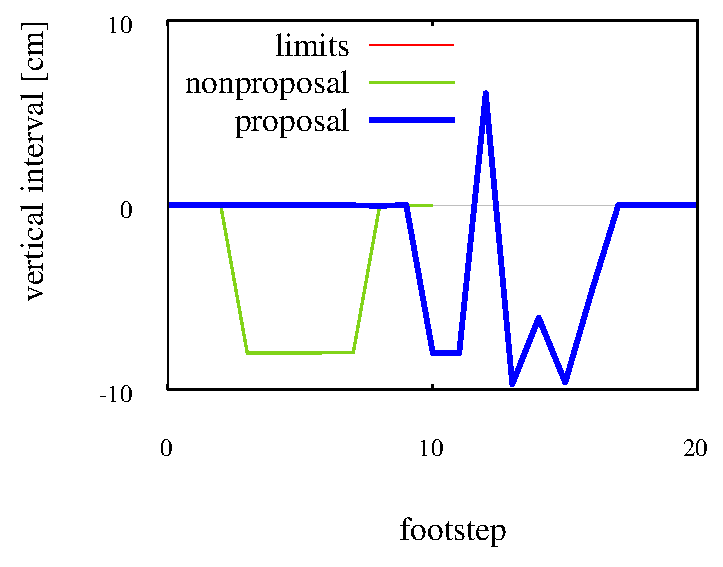
\includegraphics[width=0.75\linewidth, clip]{./figure/sim_hrp2_stair_downbad_zdiff.pdf}%
        \subcaption{Reference placement}
        \label{fig:sim_hrp2_stair_downbad_zdiff}%
    \end{subfigure}\\ %
    \vfil%
    \begin{subfigure}[c]{\linewidth}
        \centering%
        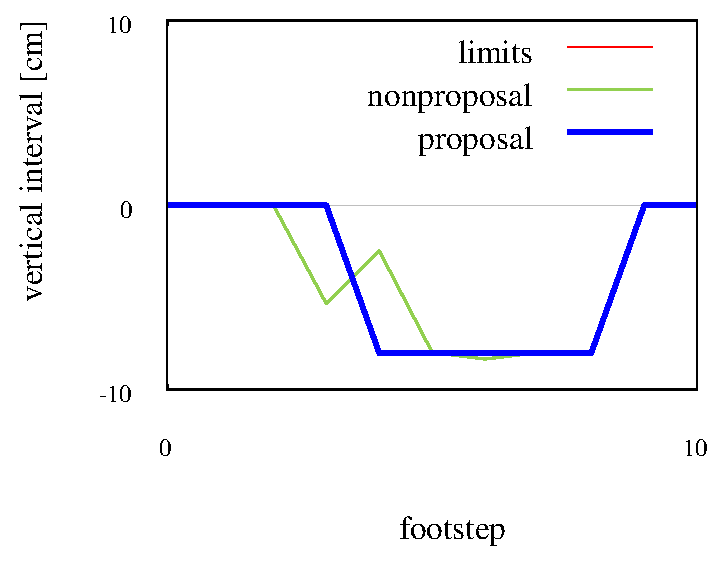
\includegraphics[width=0.75\linewidth, clip]{./figure/sim_hrp2_stair_down_zdiff.pdf}%
        \subcaption{Placement to a half step length forward}
        \label{fig:sim_hrp2_stair_downgood_zdiff}%
    \end{subfigure}%
    \caption{Vertical interval (downward stairway)}%
    \label{fig:sim_hrp2_stair_down_zdiff}%
\end{figure}
\begin{table}[pt]%
    \caption{Result of planning (downward stairway)}%
    \label{tab:sim_hrp2_stair_down}%
    \centering%
    \begin{tabular}{ccccc}%
        \toprule%
                            &   $k_{\init}$ &   $k$     &   iteration   &   time$(\ms)$ \\%
        \midrule%
        plane               &   $6$         &   $6$     &   $12$        &   $1.82$ \\%
        reference           &   $6$         &   $11$    &   $164$       &   $62.91$ \\%
        half step forward   &   $6$         &   $6$     &   $14$        &   $2.00$ \\%
        \bottomrule%
    \end{tabular}%
\end{table}

\section{本章のまとめ}
本章では,HRP-2に基づいたパラメータを用いて,
連続的変化のある地形と不連続な地形とでいくつかの問題設定で計画を行った.
そして,不連続な地形上では計算が不安定化してしまう問題が残るが,
連続的な地形では安定して最適化された脚配置計画を得ることができ,
またいずれにおいても計算時間は両脚支持期間よりも短く,
実時間性を有していることが示された.


\end{document}
